\subsection{Heterogeneous sensor systems}
\label{ch:proc_hetero}
Heterogeneous sensor systems have been an active research topic in the last decades. They can be described as a collection of sensors in the same domain that are measuring different physical properties or the same properties using different methods \cite{buczak1998self}. The majority of research is aimed to enable a self-organization of networks of heterogeneous sensors, or combine the data of heterogeneous sensors in a meaningful fashion. For capacitive proximity sensors another factor of heterogeneity has to be considered - the vastly flexible shape and material of the electrodes. This allows to create ensembles of capacitive sensors in a single domain that serve different purposes, e.g. large electrode sensors that detect the presence of a body over a longer distance combined with small electrode sensors in a specific area to detect touches. The more traditional approach combines the data generated by different categories of sensors in a meaningful fashion, to create higher level information that would not be available otherwise. One example of this approach is the previously presented LaZMouse by Smith, that added palm proximity sensing to a typical computer mouse \cite{smith1999thesis}.

In this section I will present two different contributions. The first is a concept for a heterogeneous capacitive sensor array that combines large electrode sensors to detect the presence and configuration of limbs and numerous densely packed small electrodes enabling gestural finger interaction. The second system aims at alleviating the inability of capacitive proximity sensors to clearly identify touches if the electrodes are at a distance from the touch surface. Data acquired from a microphone listening for the acoustic effects of a finger touching the surface are combined with capacitive proximity sensor data, to combine mid-air interaction and touch recognition.
\subsubsection{Heterogeneous capacitive arrays}

\begin{minipage}{\linewidth}
\centering
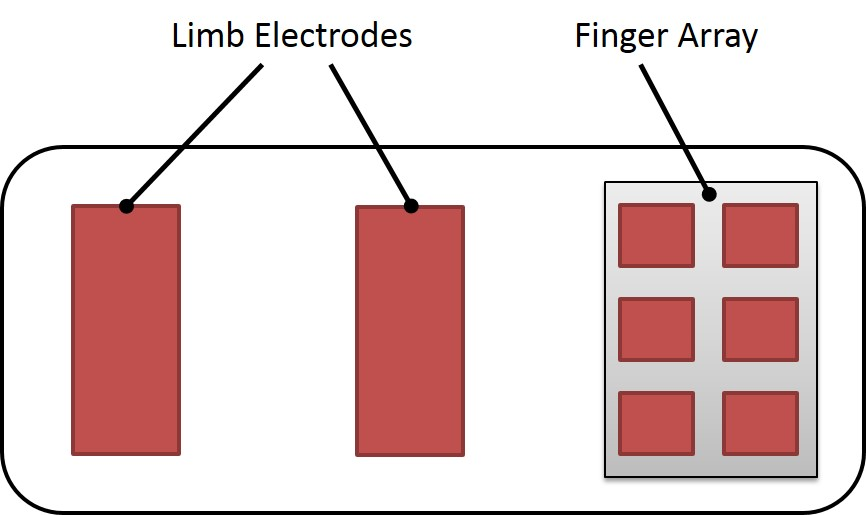
\includegraphics[width=0.7\textwidth]{images/proc_hetero_array}
\captionof{figure}{Heterogeneous sensor array for limb detection and finger tracking}
\label{fig:proc_hetero_array}
\end{minipage}

An often-cited issue of mid-air interaction systems is discriminating between an intended gesture and arbitrary movements in the detection area \cite{hinckley1994survey}. While traditionally used for full-body gesture systems, this is also true for capacitive proximity sensors that provide 3D tracking. If the interactive zones are to be integrated in design features that serve multiple purposes, there need to be methods that distinguish between typical use and intended interaction. In a project with students Sönke Schmidt and Stephan Neumann I developed a concept for a car armrest equipped with a capacitive finger interaction system \cite{braun2013ActiveArmrest}. A regular car armrest is augmented in a way that integrates the capacitive sensors in an invisible fashion. In this case it is necessary to clearly distinguish between intended control gestures by the driver or if he is just resting the arm. The idea is to use the status of both arm and hand to identify the intention. The system is using a heterogeneous combination of capacitive proximity sensors. Sensors in the middle and back of the armrest are used to detect the current status of the arm, while an array of smaller electrodes in the front can track a variety of finger gestures. The setup is shown in Figure \ref{fig:proc_hetero_array}. 

\begin{minipage}{\linewidth}
\centering
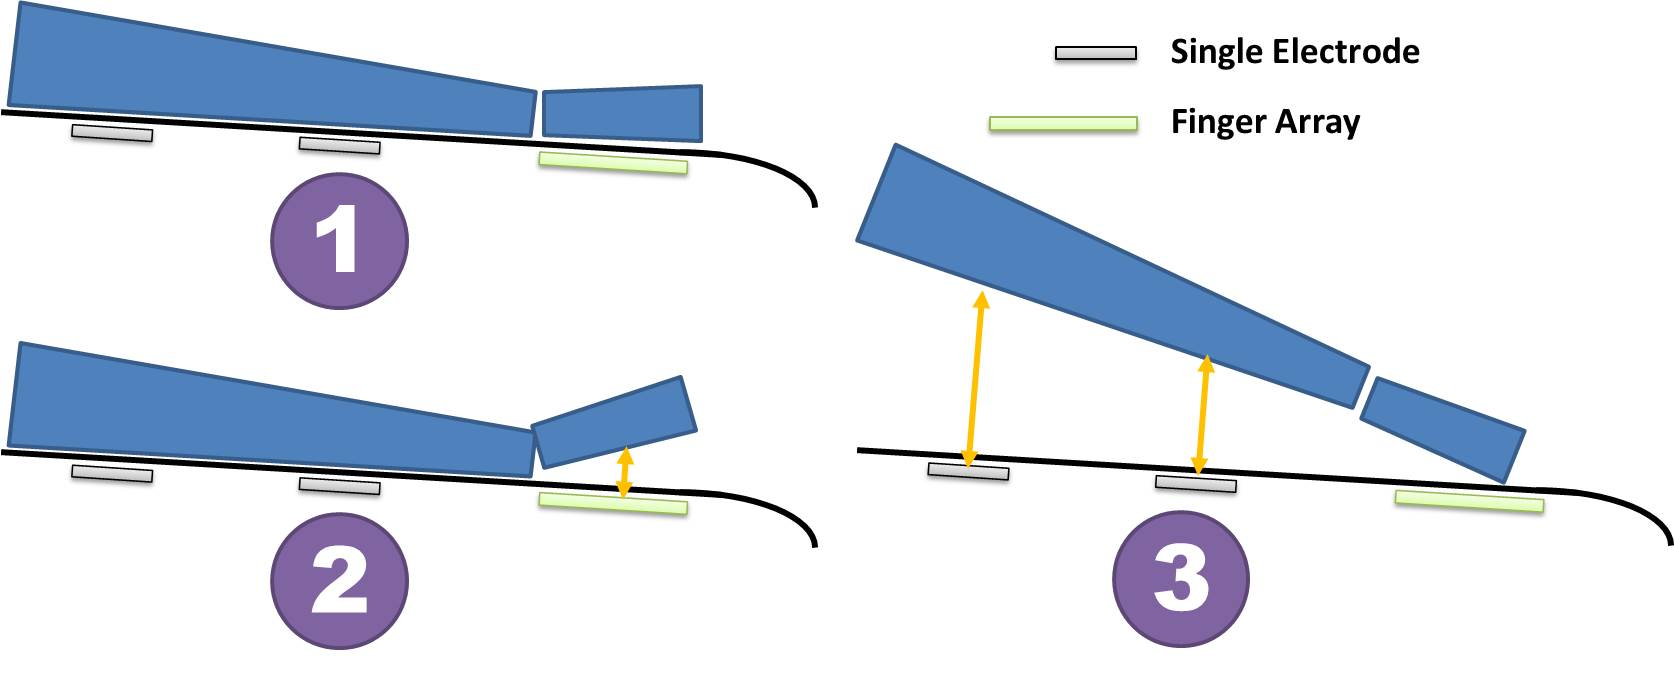
\includegraphics[width=0.8\textwidth]{images/proc_hetero_postures}
\captionof{figure}{Arm model and detection of posture based on distances to two sensors and finger array for resting position (1), hand raised position (2) and arm raised position (3)}
\label{fig:proc_hetero_postures}
\end{minipage}

In Figure \ref{fig:proc_hetero_postures} three different positions are shown that arm and hand can have on the armrest. 
\begin{enumerate}
\item Arm and hand are in resting position with both close to the surface
\item Arm resting on the back and the hand hovering in proximity of the front area
\item Arm raised position and fingers touching the front of the armrest
\end{enumerate}
The latter two positions are suitable for finger-based gestural interaction as they can be moved freely. The system should therefore be able to distinguish between the three different positions and consider either position (2) or (3) or both as intended interaction. Different interaction patterns have to be chosen for both active positions. Regarding the arm raised position the person will typically want to interact using familiar touch gestures. In the hand raised position it is necessary to track gestures that are performed in the air. In both cases we assume that a single finger is used.  
 
The data processing of the system therefore requires three distinct steps. At first the three specified limb postures have to be identified. Afterwards, the position of the fingers in or above the interaction area have to be calculated, and finally a time-series analysis of subsequent positions has to be performed, in order to infer different gestures. The two distinct arm sensors are able to determine single distance values. In addition the aggregated data of the finger detection array in the front is used to detect a third distance value. To map the different postures, a set of thresholds is used that determine if arm or hand are touching the armrest surface, or if they are hovering above it. Be $r_b$ the value of the sensor in the back, $r_m$ the value of the sensor in the middle and $r_f$ the aggregated value of the sensor values in the front $r_{f,i}$. Using three threshold levels $t_b$, $t_m$ and $t_f$ the different postures $p\epsilon{1,2,3}$ can be determined as follows
\begin{align}
r_f&=\sum^n_{i=0}{r_{f,i}} & p&=\left\{ \begin{array}{c}
1,\ \ \ r_b\ge t_b \wedge r_m\ge t_m \wedge r_f\ge t_f\\ 
2,\ \ \ r_b\ge t_b \wedge r_m\ge t_m \wedge r_f< t_f \\ 
3,\ \ \ r_b< t_b \wedge r_m< t_m \wedge r_f\ge t_f \end{array}
\right.
\end{align}
As we are acquiring sensor data proportional to distance it is also possible to calculate orientation angles of the arm and use it as input. However, for now this was not followed up any further.
The calculation of the finger position in three dimensions is adapted from the previously introduced method for sparse capacitive arrays to track objects in three dimensions that uses a combination of weighted average for planar location and stepwise linear interpolation to determine the height. 

To classify the gestures we are using points from a distinct start to a distinct stop. In case of the free-air interaction this is determined by the finger moving in a constrained part of the interactive area. In case of the touch interaction it is determined  by a finger starting and stopping to move, while exceeding a threshold indicating touch. The points between start and stop position are normalized and we are using a SVM classifier to detect the trained gestures. There are distinct classifiers for the two different methods that are triggered according to the selected interaction pattern. The SVM is trained using the sequential minimal optimization method by Platt \cite{platt1999fast}.

\subsubsection{Heterogeneous sensor fusion}
\begin{minipage}{\linewidth}
\centering
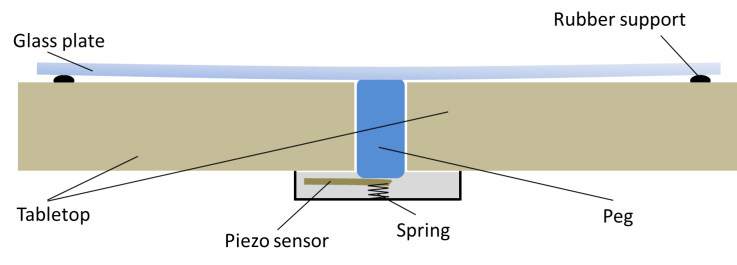
\includegraphics[width=0.8\textwidth]{images/captap_peg}
\captionof{figure}{Suspended peg knock detection system}
\label{fig:captap_peg}
\end{minipage}

As previously mentioned capacitive proximity sensors inherently lack the ability to detect touches if the electrode is at a distance from the touch surface. This may be overcome easily in systems that are tuned to work in close proximity, e.g. SmartSkin \cite{rekimoto2002smartskin}. Another option is adding a different sensor category specifically for detecting touches. The pressure applied to the surface can be detected by a suitable sensor, e.g. by using a surface suspended on sensors, such as the weight-aware dining table by Chang et al. \cite{chang2006diet}. However, this requires a specific construction and can't be retrofitted to existing systems. Additionally, there are restrictions to the potential rigidity. A different effect of surface touches is the acoustic response. A microphone connected to the surface can detect a variety of different touch events. Harrison et al. presented a system that detects varieties of fingernail scratches performed on a rough surface \cite{harrison2008scratch}. The system was later extended to detect impact events by different parts of a finger or pens \cite{harrison2011tapsense}. 

In collaboration with Sebastian Zander-Walz and Stefan Krepp I have tested different methods to combine sensors for dedicated touch detection and capacitive hand tracking integrated into an existing living room table, thus providing a potential to retrofit existing pieces of furniture \cite{Braun2013captap}. A first idea was to use a single piezo sensor to detect vibration of a glass plate that covers a living room table. The concept is shown in Figure \ref{fig:captap_peg}. This first system was prone to outside influence and had difficulties detecting multiple touch events. The second iteration used a microphone system similar to the concept provided by Harrison. However, it was extended to distinguish both impact events and different swipe varieties in a single module. The basic idea is to analyze the acquired acoustic signals in the frequency domain and use a classification method based on a number of selected features related to frequency. The supported gestures and the associated FFT profiles are shown in Figure \ref{fig:alltouch}.

\begin{minipage}{\linewidth}
\centering
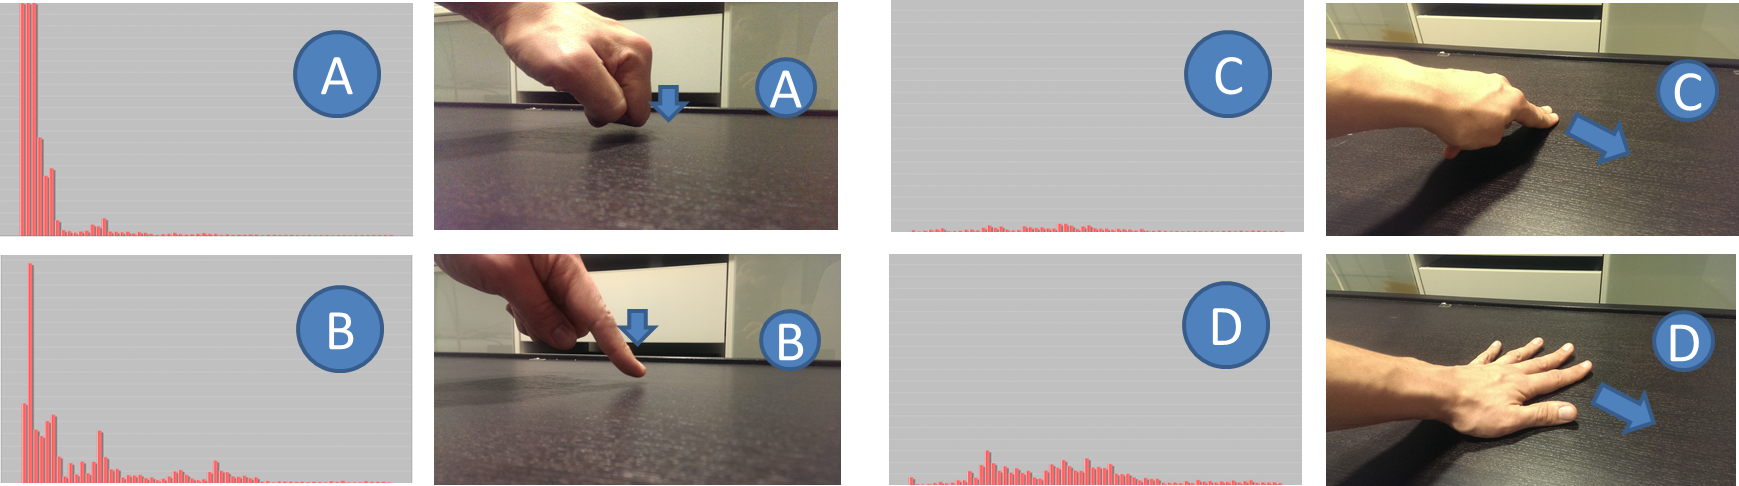
\includegraphics[width=1.0\textwidth]{images/alltouch}
\captionof{figure}{64 sample FFTs and photo for a knock event (A), a finger tap (B), a finger swipe (C) and a hand swipe (D)}
\label{fig:alltouch}
\end{minipage}

At first the audio signal is acquired using a 96kHz sample rate and a feature extraction rate of 375Hz (using a  Hanning type sliding window of 4096 (and 256 samples overlapping) samples per extraction. In order to perform a classification over this signal a variety of different features are considered. The signal differences are most significant in the frequency domain, thus we are performing a FFT over 4096 samples, looking at the first 512 of 2048 magnitude values, thus covering the frequency range up to 12kHz. We are collecting the mean value, the standard deviation and the index of the highest value within the frequency range. This process is repeated for a downsampled FFT of 64 values, similar to the method used by Harrison et al. Another frequency domain-feature we are using is the centroid, i.e. the weighted mean of the present frequencies. Additionally, we are using two time-domain features, the RMS power (root mean square), i.e. the average magnitude within the current frequency band and the number of zero crossings of the signal.

\begin{minipage}{\linewidth}
\centering
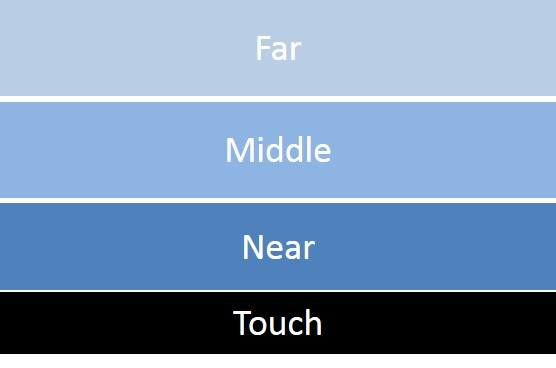
\includegraphics[width=0.5\textwidth]{images/captap_layer_interaction}
\captionof{figure}{Multiple interaction layers}
\label{fig:captap_layer_interaction}
\end{minipage}

As previously mentioned there are several limitations of free-air gesture interaction systems, related to user fatigue \cite{Baudel1993,lenman2002}. Additionally, the achievable resolution of the area above the surface of the capacitive proximity sensors is considerably lower than on the plane. If these two aspects are combined, an interaction pattern that includes a tactile sensation for improving selection events in graphical user interfaces and a sparse quantization of the interaction space above the surface seems viable. Thus we are proposing a layer-based interaction for capacitive proximity sensor devices that is comprised of a touch layer that can be used to register several different types of touch events and three different distance layers based on the proximity of the hand \cite{Braun2013captap}. This is inspired by similar multi-layer patterns introduced by Subramanian et al. for pen-supporting tabletop interaction systems \cite{subramanian2006multi}. The different layers in Figure \ref{fig:captap_layer_interaction} are intended for touch and free-air interaction. The touch layer at the bottom of the Figure represents the interaction on the surface of the table. The layers on top are formed by dividing the area above the table in three equally large parts – the near layer, the middle layer and the far layer, realized using the elevation calculation presented in the algorithm section. Inside each layer a set of different gestures can be executed and recognized while inter-layer changes may trigger additional events. Different interaction types are used for the touch and the free-air gesture layers. Swiping and dwelling gestures are suited for the free-air gesture layers while at the touch layer tapping, double tapping and different swiping patterns can be used. These interaction types may have at each layer a different functionality.
